% incluir seus pacotes aqui
% obs: cuidado para não conflitar com os pacotes inclusos neste template.

% ---------------------------------------------------------------- pacotes
\usepackage{amsmath}                       % fórmula do kappa de Fleiss
\usepackage{tabularx}                      % tabelas com colunas de largura automática
\usepackage[shortlabels]{enumitem}         % objetivos específicos como a), b), c)...
\usepackage{microtype}                     % ajuste fino do espaçamento das linhas
\usepackage{needspace}                     % título de subseção não fica sozinho no fim da página
\usepackage{xurl}                          % endereços longos das referências quebram em qualquer ponto
\usetikzlibrary{positioning,arrows.meta}   % fluxograma da revisão (o TikZ vem da classe)

% ---------------------------------------------------------------- ajustes
% links sem moldura colorida e metadados do PDF
\hypersetup{
  hidelinks,
  pdftitle={Rastreamento por terceiros em aplicativos móveis governamentais brasileiros},
  pdfauthor={Claudio da Aparecida Meireles Filho}
}

% folga extra para evitar linhas que ultrapassam a margem
\setlength{\emergencystretch}{1.5em}

% sem hifenizar "discussão" (o título da Seção 4 fica numa linha só) nem os
% nomes próprios que as regras do português dividiam errado ("Go-ogle")
\babelhyphenation[portuguese]{discussão Google AndroZoo}

% as referências, quase todas em inglês, usam a hifenização do inglês (evita
% divisões como "Procee-dings" e "IEE-E"); as referências em português têm o
% campo language = {portuguese} no referencias.bib, e o título delas mantém a
% hifenização do português
\AtBeginEnvironment{thebibliography}{\language=\csname l@english\endcsname\relax}

% "SDKs" com o s minúsculo nos títulos que a classe põe em caixa alta (capa,
% folha de rosto, folha de aprovação e título da Seção 3.4); nos marcadores do
% PDF, o comando vira o texto simples
\protected\def\SDKs{SDKs}
\pdfstringdefDisableCommands{\def\SDKs{SDKs}}

% tabelas grandes ficam no alto de uma página com texto, e não sozinhas e
% centralizadas numa página só de tabelas; se uma página só de tabelas for
% necessária, a tabela fica no alto dela
\renewcommand{\topfraction}{0.85}
\renewcommand{\textfraction}{0.1}
\renewcommand{\floatpagefraction}{0.8}
\makeatletter
\setlength{\@fptop}{0pt}
\makeatother

% fonte e nota abaixo de tabelas e figuras
\newcommand{\fonte}[1]{\par\vspace{0.6ex}{\centering\footnotesize Fonte: #1\par}}
\newcommand{\nota}[1]{\par\vspace{0.4ex}{\footnotesize\noindent Nota: #1\par}}

% rótulos fixos da classe em português (folha de rosto, folha de aprovação e
% referências); para voltar aos rótulos originais, em inglês, comente a linha abaixo
% Rótulos em português para as páginas que a classe do modelo escreve em inglês.
% A pasta configs/ não foi alterada: os comandos abaixo repetem o leiaute da
% classe (configs/idp-model.cls) e trocam apenas os textos fixos.

% texto de apresentação da folha de rosto e da folha de aprovação
\newcommand{\tipotrabalho}{Projeto de pesquisa apresentado à disciplina Projeto Capstone I}
\newcommand{\textoapresentacao}{\tipotrabalho{} como requisito parcial para a
  obtenção do título de bacharel em \nomecurso{} no Instituto Brasileiro de Ensino,
  Desenvolvimento e Pesquisa (IDP).}

\renewcommand{\folharosto}{
    \clearpage
    \thispagestyle{pretext}
    \begin{flushleft}
        {\Large\bfseries\color{fundo_idp}\MakeUppercase\autornome}

        \vspace*{3cm}
        {\Large\color{fundo_idp}\MakeUppercase\titulonome}

        \vspace*{3cm}

        \noindent{\textoapresentacao}

        \vspace*{3cm}

        {\bfseries\color{fundo_idp}
        \iforientadora Orientadora
        \else Orientador
        \fi}\\
        {\nomeorientador}

        \vspace*{3cm}
        {Brasília - DF, \anonome}
    \end{flushleft}
}

\renewcommand{\folhaaprovacao}{
    \clearpage
    \thispagestyle{pretext}
   \begin{flushleft}
        {\Large\bfseries\color{fundo_idp}\MakeUppercase\autornome}

        \vspace*{3cm}
        {\Large\color{fundo_idp}\MakeUppercase\titulonome}

    \end{flushleft}
        \vspace*{2cm}

        \noindent{\textoapresentacao}

    \begin{flushleft}

        \vspace*{2cm}
        {Aprovado em \dataaprovacaoVal}

        \vspace*{1cm}
        {\bfseries\color{fundo_idp}Banca examinadora}


        {
        \vspace*{2cm}
        \vspace{1em}
        {\nomeorientador\ (\iforientadora Orientadora\else Orientador\fi) - \instorientador}

        \vspace*{2cm}
        \vspace{1em}
        {\nomemembrobancai\ (\funcaomembrobancai) - \instbancai}

        \vspace*{2cm}
        \vspace{1em}
        {\nomemembrobancaii\ (\funcaomembrobancaii) - \instbancaii}
        }
    \end{flushleft}
}

% página de abertura e título da lista de referências
\renewcommand{\capareferencias}{
    \clearpage
    \thispagestyle{empty}
    \AddToShipoutPicture*{
        \put(-3,0){
            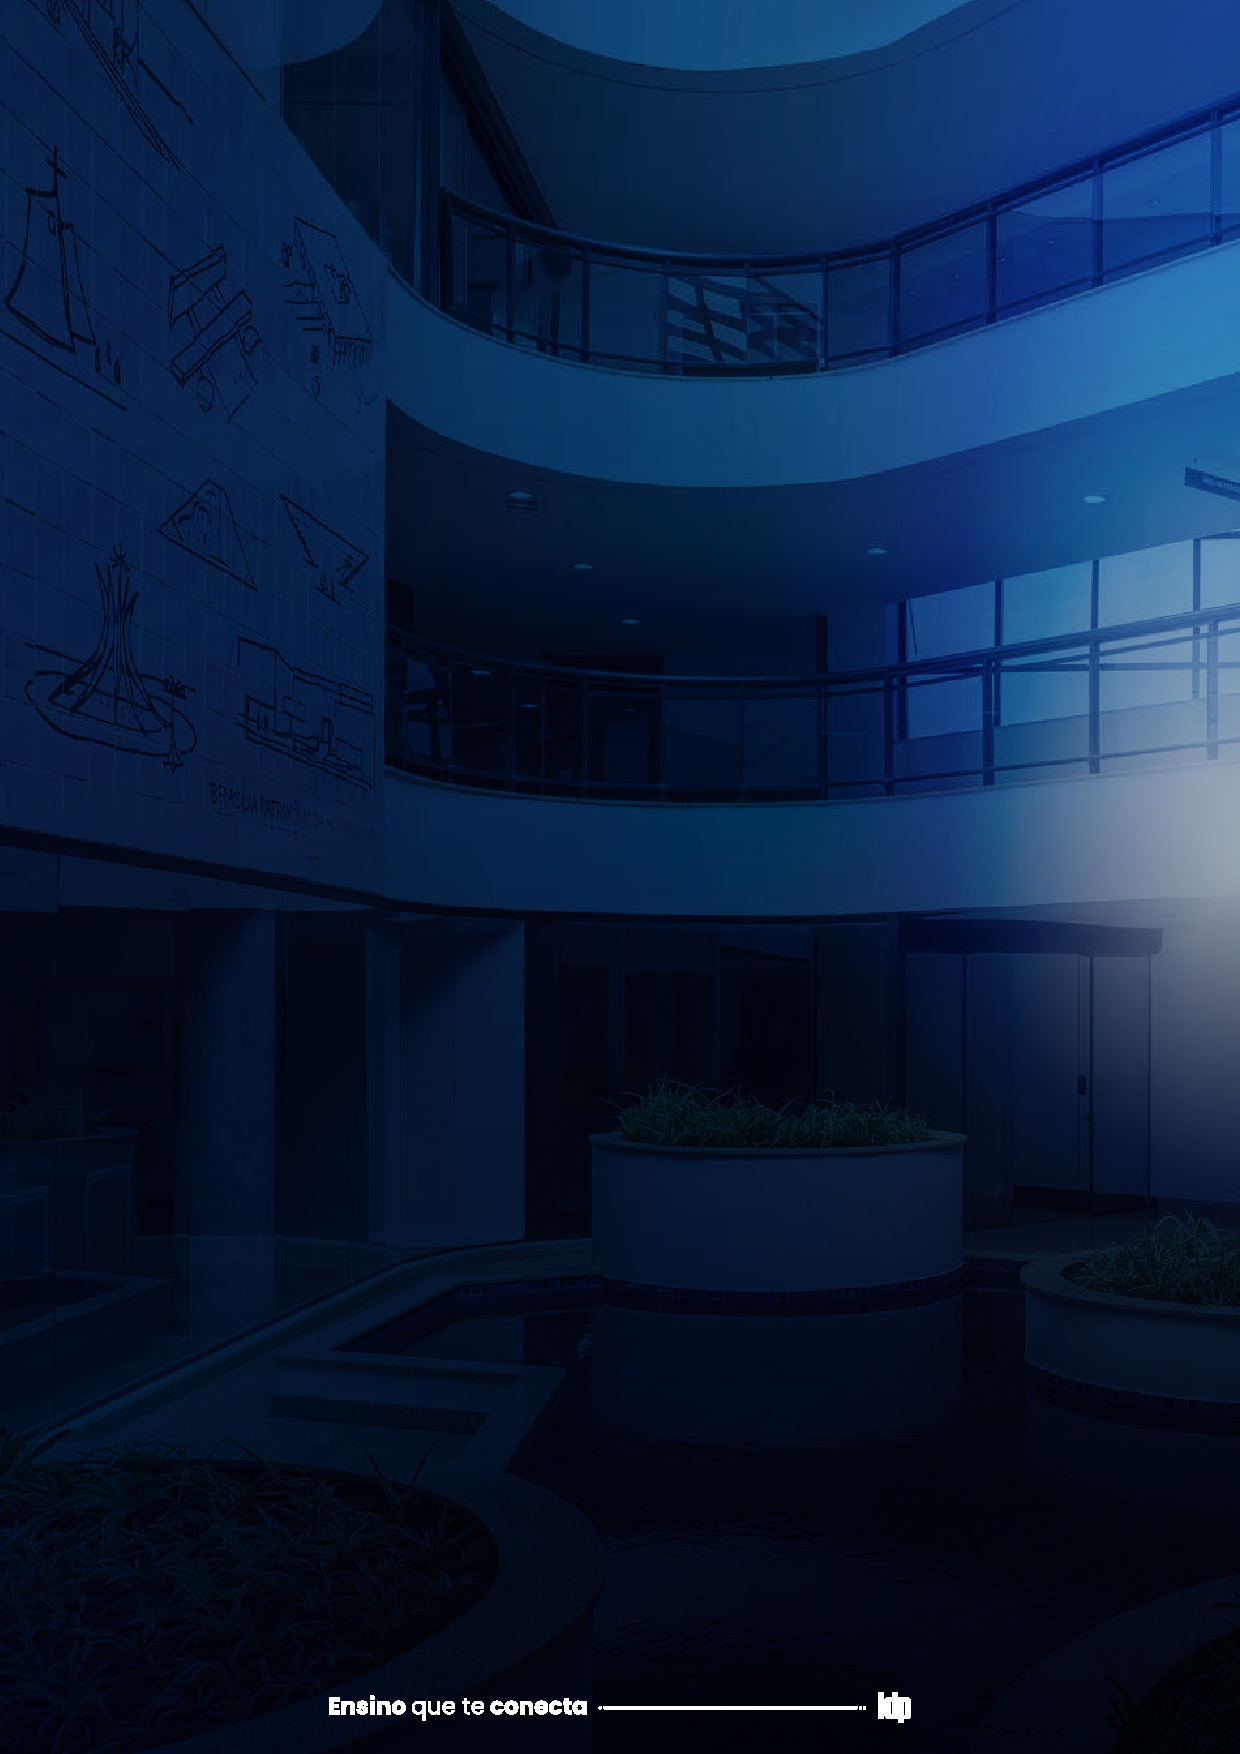
\includegraphics[width=\paperwidth,height=\paperheight]{configs/figuras/capa_secoes.pdf}
        }
    }
     \color{white}

    \vspace*{\fill}
    \begin{center}

    {\fontsize{60}{0}\bfseries\MakeUppercase{Referências}}
    \end{center}
    \vspace*{\fill}

    \refstepcounter{secnum}
    \phantomsection
    \addcontentsline{toc}{section}{Referências}

    \color{black}

    \null
    \clearpage
}

\addto\captionsportuguese{%
  \renewcommand{\refname}{%
    \color{titulos}\bfseries\MakeUppercase{Referências}
  }
}


% correção: na classe, o título de subseção e de subsubseção podia ficar sozinho
% no pé da página, com o texto começando na página seguinte; \Needspace passa o
% título para a próxima página quando não cabem ele e algumas linhas de texto, e
% \nopagebreak impede a quebra logo depois do título. O restante repete a
% definição de configs/idp-model.cls
\renewcommand{\subsecao}[1]{%
  \par\Needspace{6\baselineskip}%
  \refstepcounter{subsecnum}
  \par\vspace{1.5ex}

      \phantomsection
      \addcontentsline{toc}{subsection}{\arabic{secnum}.\arabic{subsecnum} #1}

  {\large\noindent\color{fundo_idp}\bfseries\MakeUppercase{\thesubsecnum\quad #1}}\par
  \nopagebreak
  \vspace{1ex}
}

% na subsubseção, além disso, o número ficava colado ao título no sumário,
% porque a classe escreve "\thesubsubsecnum #1" e o espaço depois do comando se perde
\renewcommand{\subsubsecao}[1]{%
  \par\Needspace{5\baselineskip}%
  \refstepcounter{subsubsecnum}
  \par\vspace{1.2ex}
  \phantomsection
  \addcontentsline{toc}{subsubsection}{\thesubsubsecnum\ #1}

  {\normalsize\noindent\color{fundo_idp}\bfseries\thesubsubsecnum\quad #1}\par
  \nopagebreak
  \vspace{0.5ex}
}
